%-----------------------------------------------------
% Template para cria��o de relat�rios da LEIC
% jlopes AT fe.up.pt, Fri May 19 09:32:24 2006
%-----------------------------------------------------
%
\documentclass[oneside,a4paper,portuges,11pt]{report}
%
%% packages
\usepackage[portuges]{babel}       % portugu�s
\usepackage{graphicx}              % images .png or .pdf w/ pdflatex OR .eps w/ latex
%\usepackage[T1]{fontenc}           % PS fonts
\usepackage[latin1]{inputenc}      % 8 bits 
\usepackage{tabularx}              % more on tables
\usepackage{picinpar}              % insert pictures into paragraphs.
\usepackage{makeidx}               % index
\usepackage{url}                   % URLs
\usepackage[pagebackref]{hyperref} %hyper-refs and back refs
\usepackage{indentfirst}           % indent first paragraph
\usepackage{setspace}
\usepackage{vmargin}
\usepackage{color}
\usepackage{fancyhdr}


%macros
\newcommand{\leic}{Licenciatura em Engenharia Inform�tica e Computa��o}
\newcommand{\feup}{Faculdade de Engenharia da Universidade do Porto}
%%BEGIN Koch
\newcommand{\foreign}[1]{\textit{#1}}
\newcommand{\nname}[1]{\textit{#1}}
%%
\newcommand{\empresa}{\textit{Novabase / Octal 2 Mobile}}
\newcommand{\projecto}{Framework de Localiza��o Passiva por Bluetooth}
%%END   Koch

\hypersetup{pdftitle={\projecto},pdfsubject={Relat�rio do Est�gio Curricular da LEIC 2006/07},pdfkeywords={},pdfauthor={Paulo Jorge Duarte K�ch},pdfcreator={wordml2latex }, colorlinks=true, linkcolor=red, anchorcolor=black, citecolor=green, filecolor=magenta, menucolor=red, pagecolor=red, urlcolor=blue, breaklinks=true, pdfstartview=FitH, pdfpagemode=UseOutlines}


%% margins
\setpapersize{A4}
%\setmargins{leftmargin}{topmargin}{rightmargin}{bottommargin}{headheight}{headsep}{footheight}{footskip}
\setmarginsrb{30mm}{20mm}{30mm}{20mm}{5mm}{10mm}{5mm}{10mm}

%%line spacing
\setstretch{1.2}           % Sets spacing different from the default 1 1/2

%% headers & footers
\pagestyle{fancy}
\fancyhead{}               % clear all fields
\fancyhead[LO]{LEIC/2005-06/Relat�rio de Est�gio} % one sided
\fancyhead[RO]{\thepage}   % one sided
\fancyfoot{}               % clear all fields
%\fancyfoot[CO]{\textit{\thepage}} % one sided
\renewcommand{\headrulewidth}{1pt}
\renewcommand{\footrulewidth}{0pt}

\setcounter{topnumber}{1}  % maximum number of floats at top of page
\setcounter{tocdepth}{2}   % sets the depth of sectional units listed in the toc


\includeonly{%
dedica,%
resumo,%
agradece,%
chapter1,%
chapter2,%
chapter3,%
chapter4,%
chapter5,%
chapter6,%
chapter7,%
chapter8,%
anexo1,%
anexo2,%
%anexo3
}

%\listfiles               % list files needed to compile this

\begin{document}

%%-- first page
\begin{titlepage}
	\begin{center}
		\vspace*{-14mm}
		{\Large \feup}\\[2mm]
		{\Large \leic}\\[18mm]
		
\includegraphics[width=56mm]{feup-logo.png}\\[20mm]
		{\Large\bf \projecto ~na\\
		 \empresa}\\[6mm]
		{\large\bf Relat�rio do Est�gio Curricular da LEIC 2006/07}\\[40mm]
		{\Large Paulo Jorge Duarte K�ch}\\[30mm]
		Orientador na FEUP: Prof.\ Prof. Jo�o Correia Lopes\\
		Orientador na \empresa: Eng.\ Eng. Jo�o Vasco Ranito\\
		\vfill %Go to the bottom of the page
		Setembro de 2007
	\end{center}
\end{titlepage}

\cleardoublepage       % an empty page                 
% Roman page numbering
\pagenumbering{roman}\setcounter{page}{1}

%%-- PREAMBLE (single-spaced)
\begin{singlespace}            
	%  Last modified on   Wed May 24 10:54:15 2006
\thispagestyle{plain}

\vspace*{80mm}
\begin{flushright}
I may not have gone where I intended to go,\\
but I think I have ended up where I needed to be.\\
--Douglas Adams
\end{flushright}

	%  Last modified on  Wed May 24 11:00:09 2006
\thispagestyle{plain}
\section*{Resumo}

Imagine-se um dispositivo \nname{Bluetooth} a ser localizado, apelidado de
\foreign{Rover}, com nenhum ou muito pouco software espec�fico, dentro de uma �rea
aonde est� instalada uma grelha de v�rios outros dispositivos de \nname{Bluetooth},
apelidados de \foreign{Beacons}. Os \foreign{Beacons} s�o estacion�rios,
� conhecida a sua localiza��o, e est�o ligados a um computador central. O
\foreign{Rover} � transportado por uma pessoa e, por isso, assume-se que tem
liberdade de movimentos total.

O objectivo deste est�gio era construir uma plataforma que dote a grelha de
\foreign{Beacons} com a capacidade de localizar o \foreign{Rover} quando este se
encontra dentro da grelha.

\textcolor[rgb]{1,0,0}{RESUMIR O RESTO DO CONTE�DO DO DOCUMENTO.}

%$\ll$M�ximo 1 p�gina ou 350 palavras.
%\vspace*{\baselineskip}
%
%``Um resumo � uma representa��o abreviada e precisa de um documento,
%sem acrescento de interpreta��o ou cr�tica, escrita de forma
%impessoal'' (ISO 214).
%
%O resumo pode ter, por exemplo, as seguintes 3 componentes:
%\begin{itemize}
%\item 1 par�grafo inicial de introdu��o do contexto geral do trabalho.
%\item Resumo dos aspectos mais importantes do trabalho descrito no presente %%relat�rio, que por sua vez documenta o trabalho mais importante realizado %%durante o est�gio. Deve mencionar tudo aquilo que foi feito, por isso deve %%concentrar-se no que � realmente importante e que deve ajudar o leitor a %%decidir se deve ou n�o consultar o restante relat�rio.
%\item 1 par�grafo final com as conclus�es do trabalho realizado.
%\end{itemize}
%$\gg$
	%  Last modified on  Wed May 24 11:03:47 2006
\thispagestyle{plain}

\section*{Agradecimentos}

%$\ll$M�ximo 1 p�gina.
%\vspace*{\baselineskip}
%
%Agradecimentos a todas as pessoas da institui��o de est�gio que
%estiveram directamente envolvidas no trabalho realizado, ou que
%contribu�ram para o seu sucesso.
%
%Agradecimentos a todas as pessoas da FEUP que de algum modo apoiaram a
%realiza��o do trabalho, ou que contribu�ram para o seu sucesso.
%
%Eventuais agradecimentos a outras pessoas, incluindo amigos ou
%familiares.
%
%Finalmente, referir e agradecer o financiamento do PRODEP (saber junto
%do secretariado da LEIC qual � o n�mero do projecto PRODEP), caso
%aplic�vel.
%
%\vspace*{\baselineskip}
%\noindent$\gg$

Agrade�o a todas as pessoas da Novabase que toleraram coabitar comigo o meu local
de trabalho, distraindo-me e ajudando-me sempre que precisei. Obrigado Daniel
Carneiro, Ricardo Afonso, Hugo Barrote, M�rio Couto e Jo�o Cavadas.

Agrade�o aos meus orientadores por todo o trabalho que envergaram e por todas as
vezes que discutiram comigo, trazendo-me sempre � terra. Obrigado Jo�o Correia
Lopes e Jo�o Vasco Ranito.

Agrade�o � FEUP por todo o meu percurso acad�mico que culminou com a oportunidade
de fazer parte de uma equipa de vida real, com problemas de vida real, dando-me
experi�ncia de vida real. Obrigado, comunidade FEUP e institui��o FEUP.

Agrade�o tamb�m ao PRODEP por todo o esfor�o desenvolvido para criar melhores condi��es
de est�gio para os estudantes do ensino superior portugu�s. Em nome de todos os estudantes,
muito obrigado PRODEP.

	\tableofcontents
	\listoffigures
	\listoftables
\end{singlespace}

\cleardoublepage                     
% Arabic page numbering
\pagenumbering{arabic}\setcounter{page}{1}

%%-- MAIN CHAPTERS
%  Last modified on  Fri May 19 09:41:45 2006

\chapter{Introdu��o}
\label{ch:intro}
\section{O projecto: Framework de radiolocaliza��o passiva por Bluetooth}
\subsection{Contextualiza��o e motiva��o}

Desde sempre que o Homem tem a necessidade de comunicar e tem sido um aspecto de
interesse permanente. Come�ou-se pela express�o corporal e sonora. Inventou-se a
comunica��o por s�mbolos, a fala e a escrita. Apareceu tamb�m a
``telecomunica��o'', comunica��o � distancia. O tel�grafo foi um dos primeiros
instrumentos de telecomunica��o. Seguiu-se o telefone e o telem�vel.

Os telem�veis, inven��o relativamente recente, t�m sido dotados de cada vez mais
capacidades. Ao que era apenas um telefone sem fios, foi-se acrescentando imensa
funcionalidade: gest�o de contactos, gest�o de agenda, leitor de m�sica digital,
etc\ldots Actualmente, com a adi��o de tanta funcionalidade, o conceito de
telem�vel est� a mudar. 

Estamos a assistir � fus�o entre telem�veis e computadores pessoais, reunindo num
s� dispositivos a capacidade de gerir e transformar informa��o, vindo do lado dos
computadores, � capacidades de comunicar informa��o, vindo do lado dos telem�veis.
Estes novos dispositivos chamam-se Assistentes Pessoais Digitais, embora sejam
mais conhecidos pelo acr�nimo em ingl�s, PDA
(\foreign{Personal Digital Assistant}).

Com toda esta funcionalidade, tem-se vindo a revelar o desejo de que estes
aparelhos, sejam PDAs ou os telem�veis mais recentes, comuniquem entre si e
possam partilhar informa��es. O \nname{Bluetooth} veio servir esta necessidade.
\nname{Bluetooth}, tamb�m conhecido como BT, � uma tecnologia de comunica��o de
dados que funciona sobre ondas r�dio, permitindo transfer�ncias de informa��o
entre dispositivos de forma c�moda e simples.

As ondas r�dio, como as que s�o usadas pelo BT, s�o propagadas pelo ar e podem
sofrer de altera��es e atenua��es durante a propaga��o. Por isso, podem ser
``sentidas'' com mais ou menos for�a pelos intervenientes nessa comunica��o.
Um aparelho interveniente nesta comunica��o precisa de estar consciente da for�a
com que v� a onda para pedir aos seus pares para a regularem conforme necess�rio.
Numa situa��o simples onde n�o haja obst�culos na propaga��o das ondas, o �nico
factor de atenua��o � a dist�ncia que a onda tem de percorrer. Se um par de
dispositivos a comunicar por BT se distanciar um do outro progressivamente,
ter�o de emitir as ondas r�dio com cada vez mais for�a para que estas cheguem
adequadamente ao seu destino.

� plaus�vel afirmar que h� alguma rela��o entre a for�a de sinal da comunica��o
entre dois dispositivos e a dist�ncia entre eles. Se um dos dispositivos for fixo,
de localiza��o conhecida, e o outro m�vel,  podemos usar esta correla��o para
determinar a que dist�ncia o dispositivo m�vel se encontra do fixo. Se tr�s
dispositivos fixos souberem esta dist�ncia, podemos saber a posi��o do dispositivo
m�vel.

Isto vai de encontro ao interesse do nosso telem�vel/PDA saber onde se encontra e
poder, potencialmente, utilizar essa informa��o. Por exemplo, mudar o volume do
aviso de chamada caso o telem�vel se encontra numa sala de reuni�es, bloquear o
nosso computador quando nos afastamos dele, s� para nomear alguns usos.

\subsection{Objectivo}

O objectivo geral deste est�gio � desenhar um sistema para localiza��o de um
aparelho, apoiando-se na correla��o entre propriedades dos sinais trocados e a
dist�ncia. Depois de desenhado o sistema, tamb�m se pretende implementar um
prot�tipo como demonstra��o de conceito.

A ideia inicial deste sistema �, num espa�o amplo, instalar v�rios dispositivos
BT fixos, formando uma grelha est�tica e bem conhecida. Cada dispositivo fixo
chama-se ``Beacon''. Um Beacon � estacion�rio, � conhecida a sua localiza��o, e
todos est�o ligados a um computador central. Al�m dos Beacons, � considerado
outro tipo de dispositivos, os ``Rovers''. Um Rover � um dispositivo BT a ser
localizado, conhecido de antem�o e �, em principio, transportado por uma pessoa.

Tendo a grelha instalada, os Beacons procuram constantemente pela presen�a de
Rovers. Quando um Beacon encontra um Rover\footnote{ Um Beacon ``encontra'' um
Rover quando se consegue ligar a ele. }, mede das propriedades dos sinais com que
� feita a comunica��o e informa o computador central dessa medida. O computador
central fica ent�o respons�vel por deduzir informa��o sobre a localiza��o dos
Rovers, a partir das propriedades dos sinais que lhe foram comunicadas pelos
v�rios Beacons. 

O sistema como um todo � composto pela grelha de Beacons e pelo \foreign{software}
de dedu��o de localiza��o.

De uma forma mais espec�fica, os objectivos do est�gio s�o, por ordem:
\begin{enumerate}
\item Averiguar as medidas que o Bluetooth proporciona, as que sejam passiveis
		de serem utilizadas como base do sistema de localiza��o;
\item Formular um sistema que use essas medidas;
\item Implementar esse sistema;
\item Confirmar a validade do sistema com testes; e
\item Determinar a precis�o/exactid�o conseguidas.
\end{enumerate}

\section{A institui��o: \empresa}

A \empresa~� uma empresa que pertence �
divis�o \foreign{Engineering} do grupo Novabase. Foi criada com o objectivo
de fornecer servi�os em dispositivos m�veis.

Na altura da sua concep��o, ainda n�o havia prolifera��o suficiente para que este
fosse um neg�cio sustent�vel. Por isso, antes de fornecer servi�os, foi preciso
criar uma base de utilizadores de PDAs razo�vel. Desde ent�o, em segundo
plano, foi-se acumulando \foreign{know-how} dentro da empresa, facilitando assim o
objectivo primordial.

Neste momento, a empresa encontra-se num ponto de viragem. O neg�cio da
distribui��o � mantido mais pelo volume de neg�cios que gera do que por interesse
estrat�gico. Agora que h� a base de utilizadores desejada, a aposta no
fornecimento de servi�os come�a a ganhar momento e import�ncia.

\section{O projecto na institui��o}

Como a empresa est� num ponto de viragem, h� que capitalizar as tecnologias
existentes nos equipamentos m�veis com o intuito de gerar valor acrescentado para
conseguir penetra��o no mercado de servi�os. Se considerarmos que quase todos os
PDAs t�m BT, aproveitando os frutos deste projecto, a empresa ter� � sua
disposi��o uma ferramenta que servir� como forte base de apoio para a cria��o de
um leque de novos produtos, gozando tanto de uma facilidade acrescida em diminuir
o \foreign{Time to Market} como de acumula��o de \foreign{know-how}.

\section{Estrutura e conte�do do documento}

Este documento est� dividido em tr�s grandes partes: apresenta��o do problema,
explana��o da investiga��o, planeamento e implementa��o da solu��o e resultados e conclus�es.

A apresenta��o do problema � feita a tr�s tempos.
No cap�tulo~\ref{ch:problema} ser� dado a conhecer ao leitor a defini��o completa do problema. Embora de forma sucinta, s�o apresentados os conceitos em que o problema assenta. Esta apresenta��o ser� devidamente guiada para que o leitor n�o tenha dificuldades em ler o resto do documento.
No cap�tulo~\ref{ch:sota} � dado a conhecer o estado da arte, a maneira como outros tentaram resolver este mesmo problema e quais os resultados a que chegaram. De todos os artigos relevantes, s�o destacados aqueles que documentam m�todos e/ou aferi��es de forma concreta.

A explana��o da estrat�gia e implementa��o da solu��o consistem em tr�s partes.
No cap�tulo~\ref{ch:investigacao} ser� apresentada a investiga��o levada a cabo para testar as v�rias hip�teses apresentadas at� agora. S�o explicadas as premissas iniciais e os processos e dedu��es que levaram at� � hip�tese final.
No cap�tulo~\ref{ch:solucao} ser� exposta a arquitectura da solu��o na sua totalidade. A an�lise � dividida na sua componente f�sica e l�gica.
Neste cap�tulo ser� exposta a arquitectura da solu��o na sua totalidade. A an�lise � dividida na sua componente f�sica e l�gica.
No cap�tulo~\ref{ch:implementacao} ser�o explicados detalhes da implementa��o. Nomeadamente, a escolha de tecnologias e dificuldades no uso das mesmas, as partes que n�o foram implementadas, o funcionamento de certas classes menos convencionais e como alterar o m�todo de localiza��o usado.


Os resultados e conclus�es est�o divididos por dois cap�tulos.
No cap�tulo~\ref{ch:resultados} ser� exposto o funcionamento comum do prot�tipo desenvolvido, ser�o avaliados os resultados do mesmo e ser�o feitas propostas de trabalho futuro.
No cap�tulo \ref{ch:conclusoes} ser� exposto o funcionamento comum do prot�tipo desenvolvido, ser�o avaliados os resultados do mesmo e ser�o feitas propostas de trabalho futuro.

%$\ll$3 ou 5 p�ginas sugeridas
%\vspace*{\baselineskip}
%%O presente documento, na sua forma actual, pretende ser um modelo
%orientador para a escrita do relat�rio final do est�gio curricular da
%LEIC, em termos de formato e de conte�do.
%Entende-se no entanto que a estrutura possa, em casos particulares,
%ser alterada de forma a relatar melhor o trabalho efectuado, devendo
%os estagi�rios acordar com os seus orientadores a estrutura mais
%adequada. 
%No Anexo A, incluem�se algumas normas a seguir na elabora��o do
%relat�rio final.
%%O corpo principal do relat�rio e os anexos n�o devem exceder os
%limites que constam no Anexo A deste documento. 
%Os anexos podem incluir textos que, embora sejam directamente
%relacionados com o trabalho, possam ser considerados como sendo
%pormenores dispens�veis numa leitura menos profunda.
%%Documentos ou prot�tipos desenvolvidos pelo autor devem sempre ser
%inclu�dos nos anexos, no mesmo volume do relat�rio ou em documento
%separado. 
%Documentos importantes produzidos ou utilizados durante o est�gio que,
%pela sua dimens�o, n�o sejam coloc�veis no corpo principal do
%relat�rio, podem tamb�m ser inclu�dos em anexos ou, simplesmente,
%apresentados como refer�ncias.
%%Nesta sec��o, ``Introdu��o'', deve descrever-se todo o contexto do
%est�gio, apresentados o tema e conclus�es do est�gio (com mais algum
%detalhe do que no resumo) e referida a organiza��o do relat�rio. 
%Deve ser apresentada a institui��o de est�gio em que decorreu o
%est�gio (tal apresenta��o � necess�ria, nesta sec��o ou em outra
%sec��o introdut�ria), o projecto e o problema concreto que o est�gio
%abordou.
%%Por exemplo, podem ser consideradas as sec��es apresentadas de
%seguida.
%%
%\section{Apresenta��o da Institui��o de Est�gio xpto}\label{sec:xpto}
%\section{O Projecto Ptox na Institui��o de Est�gio xpto}
%\section{Estudo e Desenvolvimento do Prot�tipo Toxp no Projecto Ptox}
%\section{Organiza��o e Temas Abordados no Presente Relat�rio}
%%
%\vspace*{\baselineskip}
%\noindent$\gg$

%  Last modified on   Fri May 19 09:58:40 2006

\chapter{O Problema de Radiolocaliza��o por Bluetooth}
\label{ch:problema}
Neste cap�tulo ser� dado a conhecer ao leitor a defini��o completa do problema. Embora de forma sucinta, s�o apresentados os conceitos em que o problema assenta. Esta apresenta��o ser� devidamente guiada para que o leitor n�o tenha dificuldades em ler o resto do documento.

\section{Defini��o}

O problema � construir um sistema de radiolocaliza��o passiva de aparelhos m�veis apoiado em BT. O ambiente alvo � \foreign{indoor}. Pretende-se que a localiza��o seja orientada � posi��o num local, e n�o � presen�a num local.

No sentido lato, radiolocaliza��o � o acto de localizar a posi��o de um objecto com recurso a ondas r�dio. Pode ser feita activamente ou passivamente. Activamente, o objecto analisa as ondas r�dio presentes no meio para saber onde se encontra. Passivamente, as ondas r�dio provenientes de um objecto s�o analisadas por um ou mais agentes exteriores para determinar a localiza��o desse objecto \cite{WC:Radiolocalizacao}.

Os aparelhos BT a localizar, tamb�m denominados sujeitos ou Rovers, ser�o telem�veis ou PDAs, sobre os quais n�o h� controlo. Ou seja, nestes dispositivos n�o � poss�vel fazer nenhuma altera��o de \foreign{hardware}. No m�ximo, o sistema pode requerer a instala��o de algum \foreign{software}, mas mesmo isso � indesejado. Pretende-se que o sistema consiga localizar qualquer tipo de telem�vel ou PDA. No m�nimo, a solu��o tem que funcionar com dispositivos baseado em \nname{Windows Mobile}. Nos dispositivos de apoio, denominados observadores ou Beacons, temos liberdade total, desde o \foreign{hardware} ao \foreign{software}. No entanto, deve-se tentar evitar solu��es que recorram a modifica��es de \foreign{hardware}.

\section{Background}

Para dar um melhor entendimento do conceito, ser� explicado:
\begin{itemize}
	\item A no��o de localiza��o de um objecto,
	\item O funcionamento das comunica��es r�dio,
	\item As t�cnicas de localiza��o cl�ssicas,
	\item As t�cnicas de radiolocaliza��o,
	\item A tecnologia BT, \foreign{Bluetooth}, e
	\item A aplica��o das v�rias t�cnicas de radiolocaliza��o em BT.
\end{itemize}

\subsection{Localiza��o de um objecto}

A localiza��o de um objecto � normalmente definida por uma posi��o. Uma posi��o � caracterizada por um conjunto de valores de coordenadas dentro de um sistema de coordenadas \cite{WP:Position}. Um sistema de coordenadas � geralmente definido por um ponto de origem e v�rios eixos. Cada coordenada da posi��o � referente a um eixo e representa a dist�ncia nesse eixo do ponto em quest�o � origem do referencial \cite{WP:CoordinateSystem}. Por exemplo, um dos sistemas mais conhecidos � o \foreign{World Geodetic System} \cite{WP:WGS}, o sistema de coordenadas que usamos quando referimos coordenadas de longitude e latitude.

\subsection{Ondas r�dio e comunica��o r�dio}

Ondas r�dio s�o um caso particular de ondas electromagn�ticas com frequ�ncia dentro do espectro das frequ�ncias de r�dio (entre 3 Hz e 30 GHz) \cite{WP:OndasDeRadio} \cite{WP:RadioFrequency}. Uma onda electromagn�tica � um campo electromagn�tico que viaja no espa�o, provocando oscila��es de energia por onde passa \cite{WP:RadiacaoEM}. Conv�m ter em mente que as ondas podem ser alteradas durante o seu percurso, dependendo da mat�ria com que interagem. Por exemplo: ao atravessar um vidro deformado, uma onda pode mudar de direc��o ou perder for�a; ao ``colidir'' com um determinado material, uma onda pode dissipar-se. S�o muitos os tipos de altera��es a que uma onda � suscept�vel. A susceptibilidade de uma onda sofrer uma certa altera��o depende das caracter�sticas da onda.

A comunica��o por ondas r�dio � feita por dois dispositivos: um que gera as ondas r�dio e outro que consegue detectar quando � atravessado por elas. Se associarmos um s�mbolo a um conjunto de caracter�sticas de uma onda, cada vez que o receptor detecta uma onda com essas caracter�sticas a atravess�-lo, considera que o emissor lhe comunicou esse s�mbolo \cite{WP:Radio}. Posto isto, podemos dizer que o sucesso de uma comunica��o por ondas r�dio depende de tr�s factores: a capacidade do emissor gerar ondas, a capacidade do meio transportar as ondas de forma fi�vel e a capacidade do receptor reconhecer as ondas que o atravessam. Por norma, � f�cil garantir um bom mecanismo de emiss�o e recep��o, o que normalmente apresenta problemas � o meio de propaga��o do sinal.

\subsection{Localiza��o cl�ssica}

Historicamente, a localiza��o � uma componente da navega��o. Navegar � planear e executar uma viagem de um ponto de origem para um de destino. Durante a viagem, um dos actos mais importante � a localiza��o. Localizar � determinar a posi��o a que um sujeito se encontra, normalmente para verificar que a viagem est� a decorrer correctamente, aplicando as medidas correctivas necess�rias \cite{WP:Navigation}.

A ``arte'' da localiza��o foi evoluindo ao longo dos tempos. Come�aram por ser usados esquemas simples, como o reconhecimento b�sico e a navega��o estimada. Estes sempre foram usados, tanto por Humanos como outros animais, para conseguir navegar ao longo do seu meio envolvente. O reconhecimento b�sico envolve reconhecer ``algo'', seja um s�tio ou um objecto estacion�rio. Assim que � encontrado esse ``algo'', podemos dizer que nos encontramos na proximidade dele. A navega��o estimada �, sabendo a posi��o anterior, direc��o do movimento, velocidade e diferen�a de tempo, estimar a posi��o actual. Nesta t�cnica podemos tamb�m substituir a velocidade e diferen�a de tempo por dist�ncia percorrida \cite{WP:DeadReckoning}.

Com o avan�o no campo da matem�tica, apareceram as no��es de trigonometria, dando origem aos conceitos de trilatera��o e triangula��o. Apoiadas nestes dois conceitos, apareceram novas t�cnicas de localiza��o. Uma das mais conhecidas � a navega��o celestial, que recorre a sextantes \cite{WP:Sextante} (ou equivalentes), � posi��o de certos corpos celestiais e � triangula��o.

A triangula��o permite-nos determinar a posi��o de um sujeito sabendo o �ngulo a que ele se encontra de duas localiza��es conhecidas (para mais informa��o, consultar \cite{WP:Triangulation}).

\begin{figure}[t]
  \centering
  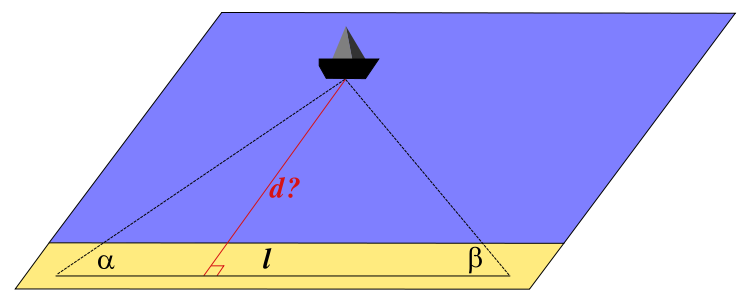
\includegraphics[width=106mm]{744px-Distance_by_triangulation.png}
  \caption{Ilustra��o de uma triangula��o.}
  \label{fig:Triangulation}
\end{figure}

Em contrapartida, a trilatera��o baseia-se em, pelo menos, tr�s posi��es conhecidas e nas dist�ncias entre cada uma destas e o sujeito a ser localizado. Cada conjunto formado por uma posi��o conhecida e a dist�ncia ao sujeito, pode ser visto como um c�rculo centrado nesse ponto conhecido. A intersec��o de tr�s destes c�rculos � a posi��o do sujeito. A grande fraqueza deste m�todo � apenas funcionar com valores perfeitos. Basta um pequeno erro em qualquer um dos valores para a solu��o se tornar imposs�vel \cite{WP:Trilateration}.

\begin{figure}[t]
  \centering
  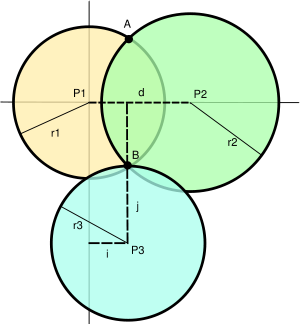
\includegraphics[width=106mm]{300px-Trilateration.png}
  \caption{Ilustra��o de uma trilatera��o.}
  \label{fig:Trilateration}
\end{figure}

Os m�todos mais recentes de localiza��o baseiam-se sobretudo na comunica��o de ondas electromagn�ticas. Um caso recente da aplica��o de uma t�cnica de localiza��o baseada em ondas electromagn�ticas � o Sistema de Posicionamento Global, mais conhecido por GPS (acr�nimo do nome em ingl�s, \foreign{Global Positioning System} \cite{WP:GPS}). Hoje em dia, este sistema � o \foreign{standard de facto} em termos de localiza��o.

\subsection{Os v�rios m�todos de radiolocaliza��o}

A descoberta das ondas electromagn�ticas trouxe novas t�cnicas de localiza��o. Embora haja um vasto leque de sistemas de localiza��o, quase todos se baseiam num conjunto base de m�todos, ou varia��es dos mesmos. Estes m�todos s�o:
\begin{itemize}
	\item Medi��o do �ngulo de recep��o do sinal,
	\item Medi��o do tempo de voo da onda e,
	\item Medi��o das altera��es na onda ao longo do voo.
\end{itemize}

A altera��o mais considerada � a atenua��o da onda. Seguidamente, cada um destes m�todos ser� devidamente explicado, analisando as desvantagens de cada um dos m�todos. Note-se que esta an�lise de contras � tendenciosa por ser feita, maioritariamente, sob o ponto de vista do problema a resolver.

\subsubsection{�ngulo de recep��o}

A idealiza��o do m�todo parece simples: descobrir o �ngulo de chegada em dois s�tios para poder triangularizar. H� v�rias maneiras de o fazer. A mais simples � ter uma antena, em rota��o constante e regular, que detecta sob qual direc��o se recebe com mais for�a o sinal emitido pelo sujeito a localizar \cite{WP:RadioDirectionFinder}. Isto pode ser feito de outras maneiras, por exemplo o uso de sistema do tipo Lorenz \cite{WP:Lorenz(navigation)} ou outras descritas em \cite{WP:AngleOfArrival}.

A desvantagem mais �bvia � n�o ser exequ�vel com antenas omnidireccionais simples.

\subsubsection{Tempo de voo}

Se soubermos os tempos absolutos que uma onda demorou a ir e vir, sabendo a velocidade de propaga��o no meio, podemos deduzir a dist�ncia. Se tr�s receptores conhecidos conseguirem determinar estes tempos, podemos localizar o sujeito por trilatera��o.

A implementa��o deste m�todo pode ser pensada de duas maneiras. Se o sujeito a localizar reflectir ondas electromagn�ticas, podemos enviar uma onda e medir quanto tempo demora da emiss�o da onda inicial at� � chegada da reflex�o da onda. O maior problema aqui � a onda ser reflectida em algo que n�o o sujeito. Nesse caso estar�amos a medir algo que n�o o sujeito.

A outra implementa��o � ser o pr�prio sujeito a emitir uma onda. Aqui, o receptor n�o sabe quando � que a onda foi emitida, s� sabe o tempo de chegada. Para ultrapassar isto, podemos redefinir ligeiramente a solu��o. Em vez de considerar s� o tempo de chegada, consideramos a diferen�a do tempo de chegada a v�rios pontos. Se soubermos 3 tempos de chegada a 3 receptores conhecidos de uma onda emitida no sujeito, calculando a diferen�a entre estes tempos, podemos deduzir tr�s hiperbol�ides. Seguindo um pensamento similar ao da trilatera��o\footnote{ Cada diferen�a de tempo de chegada da onda num par de receptores pode definir uma hiperbol�ide. Se mantivermos o pensamento da trilatera��o mas substituirmos os c�rculos por estas hiperbol�ides, temos a localiza��o do sujeito.}, temos a posi��o do sujeito. Esta implementa��o � apelidada Multilatera��o, ou localiza��o hiperbol�ide \cite{WP:Multilateration}.

O maior obst�culo em ambos os m�todos � o da medi��o de tempos. Os n�veis de precis�o e exactid�o do m�todo s�o directamente proporcionais aos existentes na medi��o dos tempos. 

\subsubsection{Altera��es no voo}

A atenua��o da pot�ncia da onda � quadr�tica ao longo do trajecto, segundo a equa��o de radar \cite{WP:Radar}. Se um receptor souber a pot�ncia de sinal da onda � sa�da do sujeito e a pot�ncia com que a recebe, podemos calcular a dist�ncia com a equa��o de radar (ou uma varia��o mais apropriada da mesma).

Aqui, o problema � saber as duas pot�ncias. Geralmente, os receptores t�m uma indica��o da for�a de sinal recebida (conhecida por RSSI, acr�nimo do ingl�s \foreign{Recieved Signal Strength Indication}). A pot�ncia emitida tem de ser dada a conhecer ao receptor de alguma maneira.

\subsubsection{Problema comum: Reflex�es}

Uma onda omnidireccional pode ser vista como uma s�rie de ondas direccionais em todos os sentidos. Se uma destas ondas for reflectida, o receptor pode ver duas vezes a mesma onda, a directa e a reflectida. A reflex�o pode ser feita por v�rios tipos de obst�culos: objectos met�licos, montanhas, etc\ldots Al�m disso, a onda directa pode nunca chegar ao receptor, chegando s� reflex�es. \cite{WP:Multipath}

\begin{figure}[t]
  \centering
  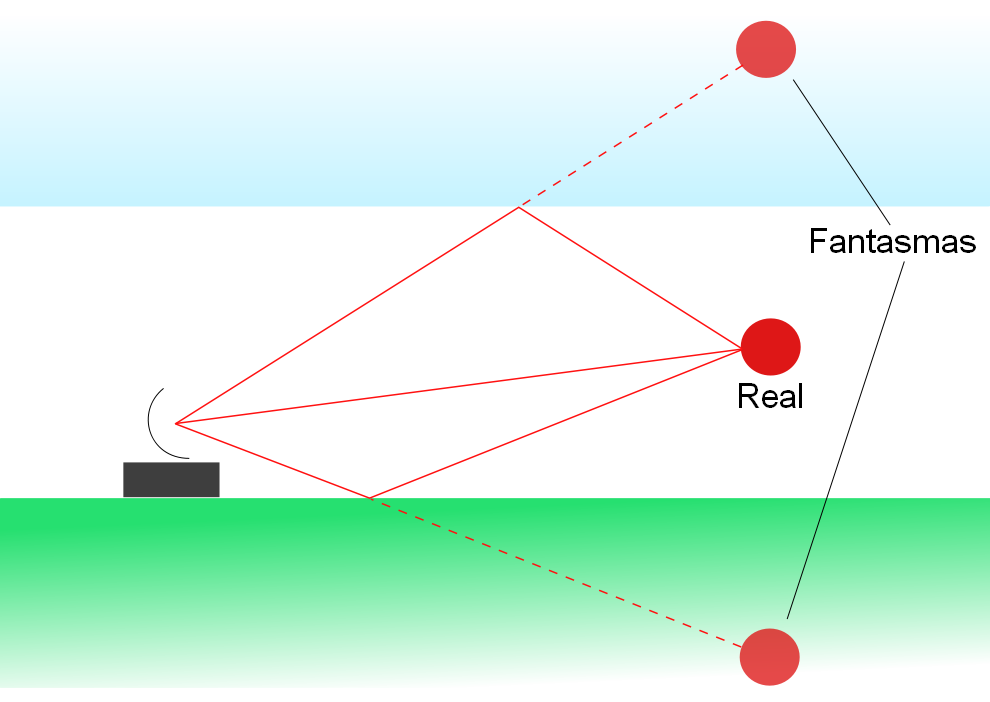
\includegraphics[width=106mm]{Multichemin.png}
  \caption{Ilustra��o de um processo de radiolocaliza��o afectado por reflex�es.}
  \label{fig:Multichemin}
\end{figure}

Nos c�lculos de �ngulo de voo, podemos ver v�rias imagens do mesmo objecto, o que pode dificultar a decis�o sobre o �ngulo.

Tanto no tempo como nas altera��es de voo, acabamos por ver v�rias recep��es da mesma onda. Se n�o ignorarmos as reflex�es, que chegam mais tarde que a onda directa, podemos pensar que, por momentos, o objecto se distanciou.

H� algumas maneiras de contrariar os efeitos das reflex�es. Por exemplo, as descritas em \cite{WP:OrthogonalFrequencyDivisionModulation} ou \cite{WP:RakeReceiver}.

\subsection{Bluetooth}

\subsubsection{Introdu��o}

\nname{Bluetooth}, tamb�m conhecido por BT, � uma especifica��o industrial para redes pessoais sem fios. O BT permite conectar e trocar informa��o entre dispositivos tais como telefones, port�teis, computadores, impressoras, c�maras digitais e consolas de v�deo jogos, sobre ondas r�dio de forma segura. A especifica��o de BT � desenvolvida e licenciada pelo \nname{Bluetooth Special Interest Group}.

O BT define o protocolo de comunica��es e o standard de comunica��o r�dio. Foi desenhado com o objectivo de ter baixos consumos, apoiando-se em emissores/receptores de custo reduzido. Os alcances variam conforme a classe do dispositivo BT (Classe 3: $\sim 1$ metro; Classe 2: $\sim 10$ metros; Classe 1: $\sim 100$ metros).

O BT permite que estes dispositivos comuniquem entre si quando estiverem ao alcance uns dos outros. Os dispositivos usam um sistema de comunica��es por r�dio e, por isso, n�o precisam de estar ao alcance visual entre eles. Podem at� estar em divis�es diferentes, desde que a transmiss�o seja suficientemente forte.

O protocolo opera na banda ISM, livre de licenciamento, na banda de frequ�ncias 2,4--2,4835 GHz. Para evitar que interfira com outros protocolos que usam esta banda, o BT divide a banda em 79 canais (cada um de 1 MHz) e alterna entre esses canais. \cite{WP:Bluetooth}

\subsubsection{Arquitectura t�pica}

Tomemos como exemplo da arquitectura da implementa��o de BT da \nname{Microsoft}, descrita no diagrama da figura X (retirado de \cite{MS:BluetoothStackArchitecture}).

Exceptuando os m�dulos de \nname{TDI} e \nname{WinSock}, todas as outras implementa��es seguem a mesma linha de pensamento.

\begin{figure}[t]
  \centering
  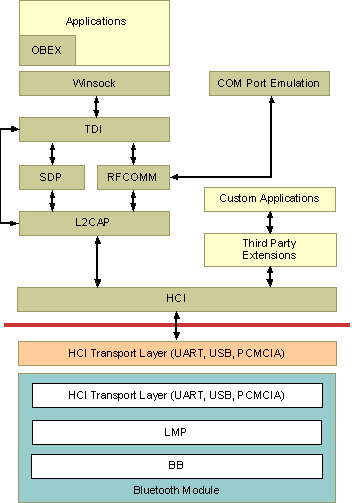
\includegraphics[width=106mm]{btstack.png}
  \caption{Arquitectura da implementa��o da \foreign{stack} de BT da \nname{Microsoft}.}
  \label{fig:BTStack}
\end{figure}

De um modo muito grosseiro podemos dividir a arquitectura em 3 grande partes: O \foreign{hardware} de BT, o HCI e os servi�os de BT.

\paragraph{Hardware Bluetooth}

O \foreign{hardware} de BT � respons�vel por implementar as tr�s partes de mais baixo n�vel de todo do sistema. Estas s�o a interface com o emissor/receptor de ondas r�dio, o controlador de canais r�dio e uma interface HCI.

A interface com o emissor/receptor de ondas r�dio � respons�vel pela manipula��o e detec��o de ondas r�dio.

O controlador de canais � respons�vel pela gest�o dos canais de r�dio. Isto passa por atender as ordens de manipula��es dos canais (estabelecer um canal, enviar dados por um determinado canal, etc\ldots). � tamb�m respons�vel por sinalizar as altera��es feitas nos canais (um canal fechou inesperadamente, h� dados � espera de serem lidos num certo canal, etc\ldots).

\paragraph{HCI}

HCI � o acr�nimo de \foreign{Host -- Controller Interface}, ingl�s de Interface Controlador -- Anfitri�o. Como o nome indica, o HCI � a interface que define o protocolo de comunica��o entre o controlador de BT e o anfitri�o onde este est� alojado. Tanto o \foreign{hardware} de BT como o sistema operativo anfitri�o t�m uma implementa��o do HCI e � atrav�s desta interface que comunicam.

Tendo em conta que toda a comunica��o de dados � feita pelo HCI, este � o denominador comum de toda a funcionalidade.

\paragraph{Servi�os de Bluetooth}

Os servi�os de BT est�o implementados do lado do anfitri�o. Todos os servi�os se apoiam, directa ou indirectamente, no HCI. H� uma grande pan�plia de servi�os \foreign{standard} dispon�veis, mas n�o s�o relevantes para a resolu��o do problema. Qualquer tipo de informa��o sobre as ondas r�dios ter� que ser disponibilizada pelo HCI. Logo, podemos ignorar todos estes servi�os e focarmo-nos na manipula��o e inspec��o do \foreign{hardware} de BT atrav�s do HCI.

\section{Radiolocaliza��o em Bluetooth}
\label{ch:problema:radiolocalizacao}

Sabendo as condi��es que o BT oferece, passaremos � an�lise da exequibilidade de cada m�todo de radiolocaliza��o.

\subsubsection{�ngulo de recep��o}

Os modelos comuns s�o todos comercializados com antenas omnidireccionais. Uma solu��o que adoptasse esta t�cnica teria de usar \foreign{hardware} espec�fico. Por ter de recorrer a \foreign{hardware} espec�fico, esta t�cnica foi posta de parte.

\subsubsection{Tempo de voo}

O HCI n�o fornece precis�o suficiente sobre a altura em que as ondas foram recebidas.

Isto poderia ser feito indirectamente com recurso a restri��es de QoS, (acr�nimo de \foreign{Quality of Service}, ingl�s para Qualidade de Servi�o). Uma liga��o pode ter termos m�nimos de qualidade associados. Se estes forem violados, o HCI deveria notificar os intervenientes na liga��o. Se pud�ssemos limitar a lat�ncia da comunica��o, de certa forma estar�amos a controlar o tempo de voo da onda. No entanto, a implementa��o de BT em alguns dispositivos \nname{Windows Mobile} s� suporta intervalos m�ltiplos de 2,5 segundos. Os valores permitidos n�o t�m uma resolu��o aceit�vel para localiza��o dentro de uma sala (em 2,5 segundos, uma onda electromagn�tica percorre 750 mil quil�metros no vazio).

N�o se tendo conseguido ultrapassar nenhuma destas dificuldades, esta t�cnica tamb�m foi posta de parte.

\subsubsection{Altera��es no voo}
\label{ch:problema:alteracoes}
O HCI tem tr�s par�metros que poderiam ser usados como base desta t�cnica: \foreign{Transmit Power}, \foreign{Link Quality} e RSSI.

O \foreign{Transmit power} � o ganho que est� presente na antena de emiss�o de ondas. Isto poderia ser interpretado como a quantidade de atenua��o que uma onda est� a sofrer. Se � preciso enviar a onda com mais pot�ncia, ent�o est� a haver mais atenua��o.

O \foreign{Link Quality} � um campo que deveria representar a qualidade da liga��o. Na especifica��o, n�o � feita nenhuma exig�ncia sobre em que caracter�sticas da liga��o este valor se deve basear. Na CSR, a \foreign{Link Quality} � medida com base no BER, (\foreign{Bit Error Rate}, ingl�s para Quociente de Erros por Bit), ingl�s para taxa de erros em bits. Se pensarmos que uma liga��o mais ``fr�gil'' (que sofre de mais atenua��o) tem mais erros por bit, h� a possibilidade de existir uma correla��o com a atenua��o e, por extens�o, com a dist�ncia.

O RSSI, tal como vem descrito na especifica��o de BT (\cite{BT:Spec}), �-nos in�til. Quando a pot�ncia de sinal recebida est� dentro dos par�metros definidos na especifica��o BT, o par�metro est� a zero. O valor sobe � medida que recebemos sinal com demasiada pot�ncia, e desce � medida que recebemos sinal com pot�ncia a menos. No entanto, os emissores s�o obrigados a manter o RSSI o mais perto do zero que conseguirem. Isto leva a que, se o RSSI desce, ambos os intervenientes subam a pot�ncia a que as ondas s�o trocadas para tentar levar de novo o RSSI a zero. Logo, esta medida vai passar a maior parte do tempo a zero.

H� um comando propriet�rio da CSR chamado RSSI\_ACL, descrito em \cite{RA:Spec}. Este comando d�, de facto, uma indica��o da for�a do sinal recebido de uma liga��o. Quanto maior a pot�ncia recebida, menor � a atenua��o. Quanto menor � a atenua��o, menor � a dist�ncia.

Estas tr�s medidas s�o claramente pass�veis de terem uma rela��o com a dist�ncia. Por exclus�o das outras t�cnicas e exequibilidade desta, � sobre esta t�cnica que ir� incidir o trabalho deste est�gio.

\subsubsection{Tratamento de reflex�es}

O HCI nunca fornece mecanismo nem de controlo nem de inspec��o directa sobre as caracter�sticas das ondas recebidas. Logo, todo o tratamento a reflex�es que houver ser� feito pelo controlador de r�dio do BT, ao qual n�o h� acesso program�tico.

\section{Resumo e Conclus�es}
Tendo estudado os m�todos dispon�veis para radiolocaliza��o passiva de apoiada em BT, chega-se � conclus�o que a �nica via que n�o foi eliminada pelos requisitos impostos ao problema � medir as altera��es durante o voo das ond�s r�dio de BT. A escolha da altera��o a ser medida pode recair sobre tr�s medidas dispon�veis: \foreign{Transmit Power}, \foreign{Link Quality} e RSSI\_ACL. Resta s� por cada uma delas � prova e optar pela mais adequada.

%$\ll$4 p�ginas sugeridas
%\vspace*{\baselineskip}
%%Este cap�tulo destina-se a efectuar uma apresenta��o do problema,
%enquadrando-o num contexto mais global. 
%S�o apresentados os pressupostos, o que se espera obter e quais s�o os v�rios
%sub-problemas em que se pode desdobrar.
%%Numa perspectiva de an�lise do problema e de previs�o de
%concretiza��o, pode incluir�se o plano de trabalhos previsto para o
%est�gio.
%%De seguida dar-se-�o exemplos de sec��es, sub-sec��es, cita��es, figuras,
%tabelas e equa��es incluindo a sua numera��o.
%%\section{Sec��o Exemplo} \label{sec:exemplo}
%%\subsection{Subsec��o Exemplo}
%%Para realizar este trabalho foram consultadas variadas refer�ncias
%bibliogr�ficas relevantes em 
%S�ries Temporais \cite{kn:Sha99},
%An�lise T�cnica \cite{kn:Geo00},
%Mercados Financeiros \cite{kn:Mur87}, e em
%E-com�rcio \cite{kn:Naf99}.
%%\section{Outra Sec��o Exemplo} \label{sec:outroexemplo}
%%Para provar:
%%\begin{equation}
%  \Big(2\sqrt{\frac{a}{b}}\Big)^m + \Big(2\sqrt{\frac{b}{a}}\Big)^m \ge 2^{m+1}
%\end{equation}
%%poderemos dividir ambos os lados da inequa��o por $2^m$, chegando a
%%\[ \Big(\frac{a}{b}\Big)^m + \Big(\frac{b}{a}\Big)^m \ge 2, \]
%%que pode ser verificada facilmente levando a:
%%\begin{equation}
%  \Big(1 + \frac{a}{b}\Big)^m + \Big(1 + \frac{b}{a}\Big)^m \ge \Big(2\sqrt{\frac{a}{b}}\Big)^m + \Big(2\sqrt{\frac{b}{a}}\Big)^m \ge 2^{m+1}.
%\end{equation}
%%\section{Outra Sec��o Exemplo}
%%O resumo dos resultados obtidos nos Est�gios s�o apresentados na
%Tabela~\ref{tab:resumo}.
%%\begin{table}[b]
%  \centering
%\begin{tabular}[t]{|l|l|cccc|c|}\hline
%\multicolumn{7}{|c|}{Pontua��es Finais}\\\hline
%Medalha & Nome            &\#1&\#2&\#3&\#4&Total\\\hline\hline
%        & Richard Feynman &25&25&25&25&100\\\cline{3-7}
%Ouro    & Albert Einstein &25&25&25&25&100\\\cline{3-7}
%        & Marie Curie     &25&24&24&25&98\\\hline
%Prata   & John Nash       &20&20&25&24&89\\\hline
%        & Jane Doe        &23&\multicolumn{2}{c}{Nenhum}&25&48\\\cline{3-7}
%Nenhuma & John Doe        &\multicolumn{2}{c}{Nenhum}&25&20&45\\\cline{3-7}
%        & Lazy Person     &5&\multicolumn{3}{c|}{Nenhum}&5\\\hline
%  \end{tabular}
%  \caption{Resumo dos Resultados de Est�gio}
%  \label{tab:resumo}
%\end{table}
%%A LEIC pretende transmitir os conhecimentos metodol�gicos, cient�ficos
%e t�cnicos que permitam satisfazer as necessidades crescentes em
%recursos humanos com educa��o superior nos dom�nios da arquitectura de
%sistemas inform�ticos e das tecnologias de informa��o e comunica��o.
%%Os licenciados pela LEIC destinam-se a integrar ou apoiar as empresas
%industriais e de servi�os, a administra��o p�blica, os laborat�rios e
%institutos de investiga��o. 
%Estes especialistas estar�o particularmente aptos a dominar os
%ambientes de desenvolvimento, utiliza��o e gest�o de sistemas e
%aplica��es inform�ticas, independentemente das realidades f�sicas a
%que estas dizem respeito.
%%Estes licenciados pela FEUP estar�o tamb�m preparados para comunicar
%com os seus colegas de outras especialidades de Engenharia,
%profissionais com grande prepara��o cient�fica. 
%Considera-se assim que � fundamental uma educa��o com uma base s�lida
%em matem�tica e f�sica, para suporte a uma pr�tica profissional que
%envolver� exerc�cios de modela��o do mundo real.
%%Surgindo na regi�o Norte de Portugal, os licenciados ir�o satisfazer o
%mercado particular dessa regi�o, onde a flexibilidade e a
%multidisciplinaridade de conhecimentos � factor importante. 
%Por tal motivo, os especialistas em software que ir�o sair deste curso
%ter�o conhecimentos de sistemas que lhes permitam resolver as
%situa��es de interface com equipamentos.
%%
%Devido �s tradi��es de ensino na FEUP e � pr�tica na regi�o Norte, os
%licenciados ter�o tamb�m a capacidade de compreender as no��es de
%gest�o essenciais para poderem vir a desempenhar fun��es de
%responsabilidade a n�vel de organiza��es, que lhes permitam lan�ar ou
%apoiar empresas com sucesso e enquadrar t�cnicos em inform�tica com
%forma��o interm�dia. 
%Pelo mesmo contexto, os licenciados tamb�m ter�o a capacidade de
%retransmitir os conhecimentos e as pr�ticas adquiridas.
%%Com vista a facilitar e potenciar a integra��o profissional dos
%licenciados, todos os alunos realizam um est�gio curricular numa
%institui��o externa no �mbito de um projecto devidamente seleccionado,
%com a dura��o de seis meses, no seu �ltimo ano do curso, sob
%orienta��o de um Professor da FEUP.
%%\section{Outra Sec��o Exemplo}
%%Na figura~\ref{fig:triangle} mostra-se o mapeamento conceptual
%utilizado na aproxima��o tradicional para provis�o de persist�ncia.
%\begin{figure}[t]
%  \centering
%  %\includegraphics[width=106mm]{triangle.pdf}
%  \caption{Mapeamento Conceptual na Aproxima��o Tradicional}
%  \label{fig:triangle}
%\end{figure}
%%\section{Resumo}
%%Neste cap�tulo foram ilustrados v�rios estilos do Relat�rio.
%%\vspace*{\baselineskip}
%\noindent$\gg$

%  Last modified on   Fri May 19 09:58:40 2006

\chapter{Estado da Arte e Trabalho Relacionado}
\label{ch:sota}

Neste cap�tulo � dado a conhecer o estado da arte, a maneira como outros tentaram resolver este mesmo problema e quais os resultados a que chegaram. De todos os artigos relevantes, s�o destacados aqueles que documentam m�todos e/ou aferi��es de forma concreta.

\section{Trabalho anterior}
H� alguma documenta��o sobre tentativas de resolu��o do problema em quest�o. Maior parte dela descreve o sucesso de um m�todo usado, mas n�o descreve o m�todo em si. No entanto, h� quatro artigos que se destacam por n�o obedecerem a essa corrente.

Em \cite{BluetoothTri} tentaram usar trilatera��o simples apoiando-se no RSSI de BT e falharam. Adaptaram uma solu��o que passou por usar hardware espec�fico. Em \cite{udana-rawcon-04} discute-se como usar o RSSI mas recorrendo a hardware ex�tico. Ambos estes casos s�o interessantes porque acabam por concluir que, sem recurso a \foreign{hardware} espec�fico, n�o conseguem deduzir posi��es apoiando-se no RSSI.

Em \cite{IndoorLocationSystems} fala-se sobre um produto comercial. No artigo analisam-se os v�rios m�todos de localiza��o e v�rias escolhas tecnol�gicas, entre estas BT. BT acaba por sobressair, sobretudo pela forte presen�a em dispositivos pessoais. A solu��o adoptada foi um misto de infravermelhos com BT. S�o apresentados os resultados conseguidos com o produto mas n�o s�o explicados os detalhes de implementa��o, pelo que n�o se consegue deduzir a ``mec�nica'' da solu��o. Ainda assim, este artigo apresenta um bom comparativo de t�cnicas e tecnologias.

Em \cite{2005-ubicomp-bluetooth} � documentada uma tentativa de construir um sistema de localiza��o baseado na an�lise do BER. � usado o sistema \nname{Active Bat} \cite{WP:ActiveBat} para recolher a posi��o real. Conclu�ram que, embora haja alguma rela��o entre o BER e a dist�ncia, n�o � suficiente para medir a dist�ncia.

Ainda de destacar, h� algumas informa��es sobre um grupo de trabalho sob a al�ada da \nname{Bluetooth Special Interest Group} para desenvolver um sistema de posicionamento local \cite{WP:BluetoothSpecialInterestGroup}. No entanto, n�o se conseguiu encontrar nenhuma informa��o sobre o trabalho desenvolvido por este grupo.

Com as restri��es do problema a ser resolvido, tendo em conta que a pesquisa levada a cabo s� encontrou estes quatro artigos relevantes, pode-se dizer com bastante ``� vontade'' que ainda n�o � conhecida nenhuma solu��o provada e bem documentada.

\section{�reas circundantes: WiFi }

Na varia��o WiFi do problema, h� algum trabalho j� estabelecido. Mesmo em artigos sobre localiza��o com BT, � muito referido um trabalho da \nname{Microsoft}: o RADAR \cite{MS:RADAR}.

O RADAR � um sistema de radiolocaliza��o para sistemas de ambientes reactivos\footnote{ Um sistema de ambiente reactivo � aquele que tem informa��o sobre o meio e age com base nela. Por exemplo, um telem�vel entrar em modo de sil�ncio cada vez que entra numa sala de reuni�es \cite{WP:ContextAwareness}.}. Usa WiFi como tecnologia de base. O principal intuito � descobrir a posi��o do sujeito para descobrir que recursos IP se encontram perto deste. Por exemplo, descobrir que impressora IP se encontra mais perto do sujeito. H� uma demonstra��o em \cite{MS:RADARDemo}.

Tendo em conta que WiFi � uma tecnologia muito presente em dispositivos \nname{Windows Mobile} (o principal alvo a atingir), se redefinirmos o problema, substituindo o uso de BT por WiFi, o sistema RADAR � uma prova concreta de exequibilidade.

O maior problema em usar WiFi � o elevado consumo de bateria. Com a cada vez maior banaliza��o do uso de perif�ricos BT (principalmente auriculares), � muito comum que os utilizadores tenham o BT ligado a maior parte do tempo. Se a solu��o desenvolvida apenas precisar que o utilizador tenha o BT ligado, � poss�vel capitalizar este crescendo de dispositivos BT ligados.


\section{Resumo e Conclus�es}
Foi encontrado muito pouco trabalho anterior que obdecesse aos requisitos impostos na formula��o do problema. Mesmo tendo o uso de WiFi como alternativa, o consumo compulsivo de bateria por parte do WiFi torna essa op��o muito pouco atraente.

%$\ll$15 p�ginas sugeridas
%\vspace*{\baselineskip}
%
%Cap�tulo de tamanho muito vari�vel com o tipo de trabalho\ldots
%
%Este cap�tulo tem como objectivo apresentar o estado da arte na �rea
%circundante do problema em causa. 
%No final do cap�tulo, o leitor deve possuir uma ideia clara acerca das
%eventuais solu��es existentes para o problema ou para problemas
%semelhantes e acerca das tecnologias que podem ser usadas, com que
%vantagens/desvantagens, no desenvolvimento do prot�tipo.
%
%
%\section{Solu��es Existentes ou Semelhantes (se aplic�vel; substituir por t�tulo apropriado)}
%
%Apresentar, se existirem, algumas solu��es conhecidas para o problema
%ou para problemas semelhantes; inclui cr�tica qualitativa/comparativa. 
%Esta apresenta��o deve justificar a necessidade de desenvolvimento da
%solu��o proposta.
%
%\section{Tecnologias a Considerar (substituir por t�tulo apropriado)}
%
%Apresenta��o das v�rias tecnologias com potencial envolvimento no
%desenvolvimento do trabalho.
%
%\vspace*{\baselineskip}
%\noindent$\gg$
%  Last modified on   Fri May 19 09:58:40 2006

\chapter{Descri��o Detalhada da Solu��o Proposta/Especifica��o (substituir por t�tulo apropriado)} \label{ch:sol}

$\ll$20 p�ginas sugeridas
\vspace*{\baselineskip}

Este cap�tulo tem como objectivo especificar a solu��o proposta. 
Deve iniciar-se com a necess�ria apresenta��o gen�rica, descendo aos
pormenores � medida do que se for sentindo como sendo necess�rio.

Os pormenores de implementa��o devem ser deixados para o cap�tulo
seguinte.

\vspace*{\baselineskip}
\noindent$\gg$



%  Last modified on   Fri May 19 09:58:40 2006

\chapter{Desenvolvimento do Prot�tipo (substituir por t�tulo apropriado)} \label{ch:prototipo}

$\ll$30 p�ginas sugeridas
\vspace*{\baselineskip}

Com este cap�tulo pretende-se que seja explicado como foi efectuada a
implementa��o do prot�tipo. 
Devem ser dadas explica��es acerca dos problemas encontrados,
previstos e imprevistos, e das respectivas solu��es.

Eventualmente, se esse for o caso, devem ser anotadas as diferen�as de
realiza��o relativamente ao planeamento efectuado no cap�tulo
anterior.

\vspace*{\baselineskip}
\noindent$\gg$


%  Last modified on   Fri May 19 09:58:40 2006

\chapter{Implementa��o do Prot�tipo}
\label{ch:implementacao}

Neste cap�tulo ser�o explicados detalhes da implementa��o, nomeadamente, a escolha de tecnologias e dificuldades no uso das mesmas, as partes que n�o foram implementadas, o funcionamento de certas classes menos convencionais e como alterar o m�todo de localiza��o usado.

\section{Escolha de tecnologias}


\subsection{Beacon}


Antes sequer de se testar as medidas como foi feito no cap�tulo \ref{ch:investigacao}, foi preciso criar um ambiente que permitisse acesso ao HCI.

A primeira tentativa de criar este ambiente foi em \emph{Windows Mobile 4}. Criar um ambiente neste Sistema Operativo (ou SO) era particularmente �til devido � disponibilidade de equipamentos com este SO. No entanto, a biblioteca dispon�vel e respectiva documenta��o s�o relativamente complexas. Por isso, n�o se conseguiu criar o ambiente necess�rio.

A pr�xima hip�tese era criar o ambiente em \nname{Windows}, tendo em conta a ampla disponibilidade com computadores com este SO. A �nica maneira de aceder ao HCI � em \nname{Kernel Land}, em \nname{Drivers}. Logo, tendo em conta o investimento consider�vel que teria que haver para construir um \nname{Driver} espec�fico para esta tarefa, foi abandonada a hip�tese.

Embora tamb�m haja algumas ferramentas para comunica��o com o HCI em \nname{Java}, todas as tentativas, em ambiente \nname{Windows}, falharam.

Em \nname{Linux}, h� uma \foreign{framework} de BT chamada \nname{BlueZ}. Esta \foreign{framework} permite acesso relativamente simples, embora trabalhoso, ao HCI.

Havia ainda a hip�tese de usar \nname{OS X}, o SO da \nname{Apple}. Seguir por esta hip�tese obrigaria a que o custo de cada Beacon fosse consideravelmente mais elevado, comparado com o uso de \nname{Linux}. Uma pesquisa breve n�o revelou nenhum resultado relevante, pelo que tamb�m se abandonou a hip�tese.

No final, a �nica alternativa era usar BlueZ. Foi nesta \foreign{framework} que assentou todo o trabalho na componente do Beacon.

\subsection{Central}


Do lado do Central, a tecnologia usada � toda assente em \nname{.NET}. Havia imensas possibilidades para a implementa��o deste sistema, tendo em conta que a �nica restri��o era conseguir ler dados de uma rede \nname{Ehternet}.

A escolha acabou por recair sobre \nname{.NET} porque:
\begin{itemize}
\item Havia um IDE relativamente poderoso (\nname{Visual Studio 2005}) dispon�vel para uso;
\item A tecnologia � madura o suficiente para j� existirem muitas bibliotecas testadas e usadas com sucesso; e
\item Acima de tudo, o estagi�rio tinha ao seu dispor a ajuda de dois colegas muito experientes em \nname{.NET}.
\end{itemize}

A linguagem de programa��o usada foi \nname{C\#}, devido � vasta experi�ncia do estagi�rio em \nname{Java}, pois \nname{Java} e \nname{C\#} s�o muito parecidos.

A persist�ncia de dados foi conseguida atrav�s do uso de \nname{NHibernate}. Esta \foreign{framework} permite que, apenas adicionando algumas anota��es, o acesso � base de dados seja todo abstra�do e automatizado, inclusive a gera��o do esquema de dados \cite{NHibernate.org}.

Para interface com o utilizador no pacote \cname{Visualizer}, foi usado \nname{Windows Forms}.

\section{Dificuldades no uso da Framework BlueZ}


Al�m do processo moroso de disposi��o f�sica dos dispositivos, um dos aspectos que mais atrasou o desenvolvimento foi a adapta��o � \foreign{framework} BlueZ. A \foreign{framework} esconde e/ou abstrai pormenores do funcionamento do BT para simplificar o pensamento do programador. Esta abstrac��o nem sempre � ben�fica ou, sequer, bem implementada. Um dos casos mais not�rios � o dos \foreign{timeouts} no estabelecimento das liga��es. Como a \foreign{framework} n�o tem documenta��o al�m do c�digo em si, todo o esfor�o inicial passou por compreender como outras pessoas usaram a \foreign{framework}.

Todas as chamadas � fun��o de cria��o de liga��es levavam um par�metro chamado \cname{to}, de \foreign{TimeOut}. No entanto, este \nname{timeout} n�o � o tempo m�ximo de espera pelo estabelecimento da liga��o, mas sim o tempo m�ximo que o c�digo espera pela confirma��o da liga��o. Isto levou a casos onde o c�digo falhava o estabelecimento da liga��o mas, inquirindo o HCI com as ferramentas certas, a liga��o era criada. S� esta confus�o atrasou imenso a implementa��o. Foi fonte de in�meras confus�es at� o estagi�rio se ter apercebido do que � que, ao certo, se estava a passar.

No fim, a ideia que passou foi a de que, para controlo preciso do HCI, � prefer�vel n�o delegar o tratamento da comunica��o, ganhando um maior controlo sobre todos os processos de BT. Para situa��es em que n�o � preciso tamanho controlo, o uso da \nname{framework} dever� ser uma vantagem.

\section{Partes n�o implementadas}


A �nica parte do sistema que n�o foi implementada foi parte da comunica��o Central --- Beacon. No prot�tipo, os dispositivos que o Beacon procurava estavam descritos em c�digo, ao inv�s de lhe serem comunicados pelo central.

De resto, foi implementada a totalidade da solu��o.

\section{Implementa��o de classes}


Nesta sec��o � explicado o funcionamento de duas classes que, embora n�o suficientemente relevante para estar na descri��o da solu��o, � importante para se perceber o funcionamento do sistema como um todo.

\subsection{Binary Map}
\label{ch:implementacao:binarymap}

O objectivo desta classe � representar uma figura geom�trica presente numa �rea de duas dimens�es atrav�s de um \foreign{array} bidimensional, como se fosse um quadriculado. A �rea que cont�m a figura � mapeada num \foreign{array} bidimensional de booleanos. Se a posi��o do \foreign{array} correspondente a uma parte da �rea mapeada contiver o valor ``verdadeiro'', ent�o essa parte da �rea pertence � figura geom�trica representada.

Um objecto desta classe tem os valores m�nimos e m�ximos de cada eixo da �rea representada, o factor de escala para cada eixo e o \foreign{array} de booleanos.

\subsection{Protocol Talker e String Machine}
\label{ch:implementacao:machine}


O tratamento da comunica��o Beacon --- Central � feito com recurso a uma m�quina de estados. A m�quina de estados em si est� implementada na classe abstracta \cname{StringStateMachine}. O objectivo desta classe � ler dados, \foreign{input}, de uma \foreign{stream} e chamar m�todos conforme o formato desses dados.

Tentando fazer um mapeamento para a defini��o te�rica de m�quina de estado temos:
\begin{itemize}
\item Alfabeto de entrada: s�mbolos ASCII.
\item Conjunto de estados: conjunto de m�todos com o atributo \cname{State}, ou equivalente. Estes m�todos t�m de obedecer ao \nname{delegate} \cname{StringStateMachine.State}. Devem devolver o conjunto de estados que ser�o aceites a seguir ao processamento deste estado. Quando a m�quina de estados entra num estado, � executado o m�todo correspondente.
\item Estado inicial: este estado est� impl�cito no construtor.
\item Fun��o de transi��o de estados: este conceito est� um pouco adulterado. Ao inv�s de receber o estado actual e o \emph{input} e devolver o pr�ximo estado, a fun��o recebe o \emph{input} e um mapa de \nname{RegEx} para fun��o, que representa as transi��es poss�veis, e devolve o pr�ximo estado. A \nname{RegEx} correspondente a um estado est� na anota��o do m�todo que o representa. Os pr�ximos estados poss�veis s�o devolvidos pelo estado anterior. Os estados poss�veis para a primeira transi��o s�o os marcados com a anota��o \cname{StartingState} (que descende da anota��o \cname{State}).
\item Estados finais: um estado � considerado final quando chama a fun��o \cname{End} durante a execu��o.
\end{itemize}

A classe \cname{ProtocolTalker}, descendente de \cname{StringStateMachine}, implementa apenas os m�todos, anotados devidamente, que devem ser chamados cada vez que chega uma mensagem do Beacon.

\section{Alternando do m�todo de localiza��o}


Para mudar o m�todo de localiza��o temos de ter aten��o a dois aspectos: onde se guardam as medi��es efectuadas e como s�o calculadas as estimativas das posi��es dos Rovers.

As medi��es efectuadas est�o guardadas em duas classes diferentes, conforme a natureza da medi��o. As medi��es Beacon---Beacon  est�o guardadas em objectos da classe \cname{Ruler}. As medidas Beacon---Rover est�o guardadas em objectos da classe \cname{Donut}. Em ambos os casos, � mantida uma lista (chamada \cname{values}) das $N$ �ltimas medi��es efectuadas, onde $N$ � um valor est�tico de cada classe (chamado \cname{BACKLOG}). O acesso a esta lista, feito atrav�s de chamadas ao m�todo \cname{GetRssi}, sup�e que apenas queremos um �nico valor; por exemplo, a m�dia das medi��es guardadas. Na implementa��o actual, a lista guarda apenas um valor e o m�todo \cname{GetRssi} devolve esse valor.

O c�lculo das estimativas est�, tamb�m, distribu�do por dois s�tios, objectos da classe \cname{Donut} e da classe \cname{PositionedRover}. Os objectos \cname{Donut} s�o respons�veis por calcular o anel, centrado no Beacon desse \cname{Donut}, onde estimam que o Rover desse \cname{Donut} esteja. Na implementa��o actual, o raio interno e externo do anel � calculado no m�todo \cname{GetRadius}, e � ai que � feita a rela��o entre as medi��es e a dist�ncia. Os objectos \cname{PositionedRover} s�o respons�veis por intersectar todos os an�is que se referem ao Rover representado pelo objecto.

\subsection{Exemplo de um c�lculo alternativo}


Sabendo que o RSSI\_ACL � logar�tmico ao longo da dist�ncia, podemos dizer que a dist�ncia � exponencial ao longo do RSSI\_ACL. A t�tulo de exemplo, suponha-se que � pretendido que a dist�ncia seja calculada com recurso a uma regress�o exponencial em vez de recorrer ao pensamento explicado em \ref{ch:investigacao:relacao}. Para isso, precisar�amos de duas modifica��es: criar um mecanismo que efectuasse a regress�o e adaptar a implementa��o para o usar.

Primeiro, seria criada uma classe respons�vel pelo c�lculo da regress�o. Esta receberia um dicion�rio, onde as chaves fossem medi��es e o valor de cada chave fosse a dist�ncia a que essa medi��o foi recolhida, e devolveria uma fun��o que representava o resultado da regress�o.

Esqueleto da implementa��o da fun��o de calculo da regress�o em C\# 2.0.
\begin{flushleft}
{\textcolor[rgb]{0,0,1}{{\scriptsize public}}~{\scriptsize  }\textcolor[rgb]{0,0,1}{{\scriptsize delegate}}~{\scriptsize  }\textcolor[rgb]{0,0,1}{{\scriptsize double}}~{\scriptsize  }\textcolor[rgb]{0.16862745098039217,0.5686274509803921,0.6862745098039216}{{\scriptsize Regression}}~{\scriptsize  (}\textcolor[rgb]{0,0,1}{{\scriptsize short}}~{\scriptsize  x);}}
\end{flushleft}
\begin{flushleft}
{\textcolor[rgb]{0,0,1}{{\scriptsize public}}~{\scriptsize  }\textcolor[rgb]{0.16862745098039217,0.5686274509803921,0.6862745098039216}{{\scriptsize Regression}}~{\scriptsize  DeduceExpRegression}{\scriptsize (}\textcolor[rgb]{0.16862745098039217,0.5686274509803921,0.6862745098039216}{{\scriptsize Dictionary}}$<$\textcolor[rgb]{0,0,1}{{\scriptsize short}}{\scriptsize , }\textcolor[rgb]{0,0,1}{{\scriptsize double}}$>$ {\scriptsize evidence)}{\scriptsize \{}}
\end{flushleft}
\begin{flushleft}
\hspace{1.2672040550529761cm}{
{\scriptsize }
\textcolor[rgb]{0,0.5019607843137255,0}{{\scriptsize //we should get something like $y = e\frac{x-B}{A}$. We want A, B and C.}}
}
\end{flushleft}
\begin{flushleft}
\hspace{1.2672040550529761cm}{{\scriptsize }\textcolor[rgb]{0,0,1}{{\scriptsize double}}~{\scriptsize  a = }\textcolor[rgb]{0,0,1}{{\scriptsize this}}{\scriptsize .CalculateA(evidence);}}
\end{flushleft}
\begin{flushleft}
\hspace{1.2672040550529761cm}{{\scriptsize }\textcolor[rgb]{0,0,1}{{\scriptsize double}}~{\scriptsize  b = }\textcolor[rgb]{0,0,1}{{\scriptsize this}}{\scriptsize .CalculateB(evidence);}}
\end{flushleft}
\begin{flushleft}
\hspace{1.2672040550529761cm}{{\scriptsize }\textcolor[rgb]{0,0,1}{{\scriptsize double}}~{\scriptsize  c = }\textcolor[rgb]{0,0,1}{{\scriptsize this}}{\scriptsize .Calculate}{\scriptsize C}{\scriptsize (evidence);}}
\end{flushleft}
\begin{flushleft}
\hspace{1.2672040550529761cm}{{\scriptsize }\textcolor[rgb]{0,0,1}{{\scriptsize return}}~{\scriptsize  }\textcolor[rgb]{0,0,1}{{\scriptsize new}}~{\scriptsize  }\textcolor[rgb]{0.16862745098039217,0.5686274509803921,0.6862745098039216}{{\scriptsize RegressionResult}}{\scriptsize (}\textcolor[rgb]{0,0,1}{{\scriptsize delegate}}{\scriptsize (}\textcolor[rgb]{0,0,1}{{\scriptsize short}}~{\scriptsize  x) \{}}
\end{flushleft}
\begin{flushleft}
\hspace{1.2672040550529761cm}{{\scriptsize }\hspace{1.2672040550529761cm}{\scriptsize }\textcolor[rgb]{0,0,1}{{\scriptsize return}}~{\scriptsize  }\textcolor[rgb]{0.16862745098039217,0.5686274509803921,0.6862745098039216}{{\scriptsize Math}}{\scriptsize .Exp(x - b / a)}{\scriptsize  + c}{\scriptsize ;}}
\end{flushleft}
\begin{flushleft}
\hspace{1.2672040550529761cm}{{\scriptsize }{\scriptsize \});}}
\end{flushleft}

{{\scriptsize \}}}

Em segundo lugar, seria alterado o m�todo \cname{GetRadius} para:
\begin{enumerate}
\item Passar por todos os objectos \cname{Ruler} e recolher a dist�ncia que cada um representa e a medi��o a� guardada,
\item Manipular a estrutura dessa informa��o para estar de acordo com o dicion�rio que a classe de regress�o requer,
\item Dar ao m�todo da classe (ou do objecto da classe, conforme a implementa��o) o dicion�rio para efectuar a regress�o, e
\item Guardar a fun��o resultante da regress�o.
\end{enumerate}

Posto isto, era s� chamar o m�todo resultante com o RSSI\_ACL do Donut para ter uma dist�ncia.

\section{Resumo e Conclus�es}
Foram apresentadas as principais decis�es da implementa��o da solu��o proposta. Por uma quest�o de conveni�ncia, a �nica parte da solu��o que n�o foi implementada foi a comunica��o do Central para os Beacons dos endere�os dos Beacons e Rovers que deveriam ser monitorados. Do lado do Beacon, toda a implementa��o foi feita em ambiente \nname{Linux}, com recuso � \foreign{framework} \nname{Bluez}. Do lado do Central, optou-se por usar .NET, devido ao vasto apoio t�cnico e social dispon�vel. Foi explicado como foram implementadas as classe \cname{ProtocolTalker}, as dificuldades de adapta��o ao uso de \nname{Bluez} e \cname{BinaryMap} e com alternar de m�todo de localiza��o.

%$\ll$30 p�ginas sugeridas
%\vspace*{\baselineskip}
%
%Com este cap�tulo pretende-se que seja explicado como foi efectuada a
%implementa��o do prot�tipo. 
%Devem ser dadas explica��es acerca dos problemas encontrados,
%previstos e imprevistos, e das respectivas solu��es.
%
%Eventualmente, se esse for o caso, devem ser anotadas as diferen�as de
%realiza��o relativamente ao planeamento efectuado no cap�tulo
%anterior.
%
%\vspace*{\baselineskip}
%\noindent$\gg$
%  Last modified on  Wed May 24 17:51:57 2006

\chapter{Resultados e Avalia��o}
\label{ch:resultados}
Neste cap�tulo ser� exposto o funcionamento comum do prot�tipo desenvolvido e ser�o avaliados os resultados do mesmo.

\section{Funcionamento T�pico do Prot�tipo Desenvolvido}


Nesta sec��o ser� retratado o funcionamento t�pico do prot�tipo desenvolvido. Come�a-remos pela instala��o das componentes f�sicas, pelos procedimentos de ``arranque'', passando pelo funcionamento pleno de todo o sistema at� ao comportamento das dedu��es efectuadas.

\subsection{Instala��o e Arranque}
\label{ch:resultados:instalacao}

O primeiro aspecto a ter em mente � o s�tio que cada Beacon ter�. Estes devem estar dispostos de modo a que todas as posi��es a monitorizar estejam cobertas pelo alcance de, pelo menos, tr�s Beacons. Assumindo que queremos monitorar a presen�a de Rovers numa sala inteira, na Figura~\ref{fig:GoodSetup} o de um bom posicionamento e na Figura~\ref{fig:BadSetup} temos um exemplo de um mau posicionamento.


\begin{figure}[t]
  \centering
  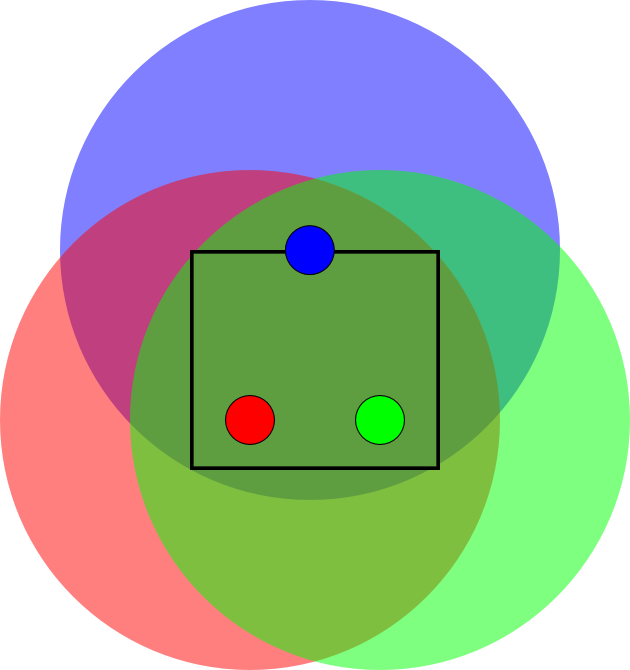
\includegraphics[width=56mm]{GoodSetup.png}
  \caption{Instala��o bem planeada se se quiser cobrir a totalidade duma sala.}
  \label{fig:GoodSetup}
\end{figure}

\begin{figure}[t]
  \centering
  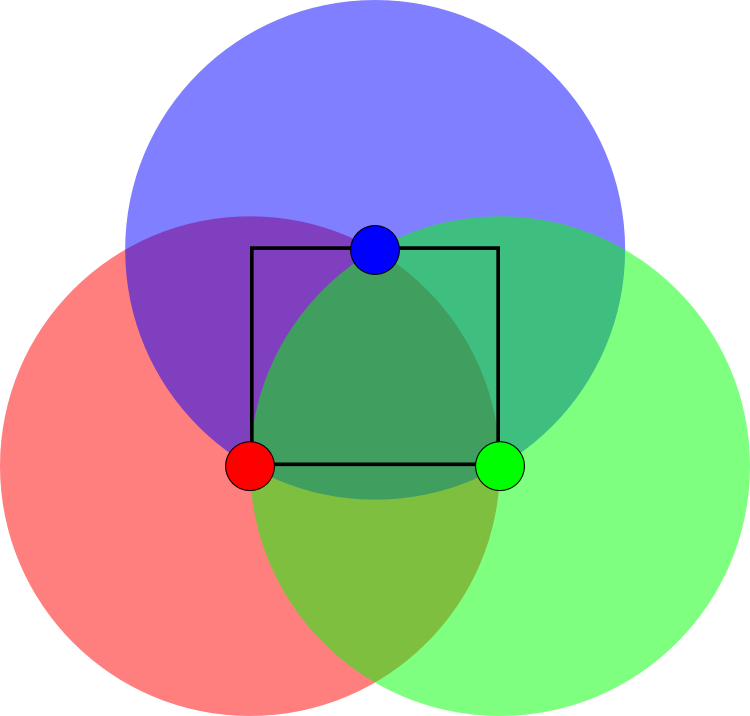
\includegraphics[width=56mm]{BadSetup.png}
  \caption{Instala��o mal planeada se se quiser cobrir a totalidade duma sala.}
  \label{fig:BadSetup}
\end{figure}

A pr�xima preocupa��o � como dispor os Beacons em si, tanto o dispositivo BT como o anfitri�o do mesmo\footnote{ Como explicado em 5.1, um Beacon como um todo � constitu�do pelo dispositivo BT e pela m�quina onde este est� hospedado.}. O dispositivo BT deve estar no s�tio planeado no passo anterior. � preciso aprovisionar s�tios para os anfitri�es e, talvez, os cabos necess�rios para ligar os dispositivos BT aos anfitri�es (caso a liga��o seja USB ou a antena do dispositivo seja externa).

Tendo os Beacons dispostos e instalados, falta lig�-los a uma rede \nname{Ethernet}. Aqui, o maior inconveniente � ter de evitar o uso de WiFi. WiFi usa a mesma banda de frequ�ncias que o BT e pode interferir na localiza��o, logo o seu uso deve ser minimizado.

O pr�ximo passo � ligar o Central � rede \nname{Ethernet} e arrancar o programa desta parte do sistema. Durante o arranque, o Central envia para o \nname{stdout} o endere�o IP e porta TCP aonde vai esperar que os Beacons se liguem. O passo seguinte � correr o bin�rio que cont�m a parte do Beacon do sistema em cada um dos Beacons, dando como argumento o IP e a porta TCP do Central.

Nesta altura, os Beacons come�am o di�logo com o Central. Primeiro avisam que come�aram uma sess�o de funcionamento. N�o muito depois, os Beacons devem come�ar a tirar medi��es de RSSI\_ACL da for�a de sinal com que se ``v�em'' uns aos outros, informando o Central dos valores.

Nesta altura, o sistema est� pronto a localizar um Rover que entre na sua �rea de actua��o.

\subsection{Funcionamento}


Se ligarmos um dispositivo BT reconhecido como Rover, eventualmente\footnote{``Eventualmente'' porque um Beacon s� pode tentar ligar-se a um Rover de cada vez e cada tentativa de liga��o demora aproximadamente 5 segundos.}, os Beacons ligam-se a ele.

No melhor dos casos, os Beacons demoram 5 segundos a reconhecer a presen�a do Rover. No pior dos casos, demoram o n�mero de Rovers registados multiplicado por cinco, em segundos. O valor m�ximo de espera por resposta de um Rover pode ser controlado. Com base em observa��es emp�ricas, abaixo dos 3 segundos, as liga��es nem sempre se concretizam e acima de 5 segundos n�o temos aumento de conectividade numa �rea de 8 metros quadrados.

� medida que as liga��es s�o efectuadas, retiradas medi��es do RSSI\_ACL e comunicado o seu valor ao Central, a interface gr�fica vai mostrando as dedu��es feitas pelo Central. Quando tr�s an�is se intersectam, � marcado na interface o centro geom�trico da �rea de intersec��o.

Na Figura~\ref{fig:Demo} temos uma imagem do \cname{Visualizer} em funcionamento. As bolas vermelha, verde e azul s�o Beacons. A bola azul claro � a estimativa actual da posi��o de um Rover. Cada anel verde � uma estimativa de um Beacon sobre um Rover. A �rea pintada a roxo � onde se espera que o Rover possa estar. Neste exemplo em espec�fico, temos s� uma liga��o entre o Rover e o Beacon vermelho.

\begin{figure}[t]
  \centering
  \includegraphics[width=106mm]{Demo.png}
  \caption{Exemplo do \cname{Visualizer} em funcionamento.}
  \label{fig:Demo}
\end{figure}

\section{Comportamento e Avalia��o das Estimativas}


Nos testes efectuados, os Beacons estavam dispostos num tri�ngulo is�sceles rect�ngulo, cada cateto com 2,5 metros.

Nos testes efectuados, o sistema, quase sempre, detectava com precis�o quando o Rover se situava no centro geom�trico do pol�gono formado pelos Beacons. � medida que o Rover se distanciava do centro, embora com menos sucesso, o sistema conseguia ``ver'' o sentido do deslocamento relativamente bem, mas n�o a quantidade do mesmo. Ou seja, o sistema sabia para que lado se mexeu o Rover, mas n�o o quanto se mexeu. As estimativas da amplitude do movimento eram sempre menores do que a amplitude real. Este desfasamento crescia � medida que o Rover se distanciava do centro.

Pelo comportamento observado, pode-se facilmente concluir que ignorar o andamento logar�tmico do RSSI\_ACL ao longo da dist�ncia foi um erro. � de notar que, mesmo com esta falha, o prot�tipo consegue estimar minimamente a posi��o de um Rover. Isto evidencia algum progresso e d� seguran�a para investir mais estudo num sistema de radiolocaliza��o passiva apoiada em BT.

\section{Resumo e Conclus�es}
Al�m de explicado o processo t�pico de instala��o e funcionamento do prot�tipo desenvolvido, neste cap�tulo conclui-se que o m�todo explicado na Sec��o~\ref{ch:investigacao:relacao} produz resultados, mas muito pouco satisfat�rios. O sistema � capaz, em situa��es muito espec�ficas de, de facto, deduzir a posi��o de um Rover.

%$\ll$5 p�ginas sugeridas
%\vspace*{\baselineskip}
%
%A exist�ncia ou n�o deste cap�tulo depende do tipo de trabalho;
%admite-se que, em alguns casos, possa ser convertido numa sec��o do
%cap�tulo~\ref{ch:prototipo} ou do cap�tulo ~\ref{ch:conclusao}.
%
%\vspace*{\baselineskip}
%\noindent$\gg$
%%%

%  Last modified on  Wed May 24 17:51:57 2006

\chapter{Conclus�es}
\label{_Ref31804431}

Neste cap�tulo ser� sumariado o conhecimento adquirido ao longo do est�gio.

A partir do trabalho realizado, podemos concluir que:
\begin{itemize}
\item N�o introduzindo hardware ``ex�tico'', com o fraco suporte para inspec��o do sinal da comunica��o BT requerido pela especifica��o, a solu��o ter� que se apoiar em extens�es propriet�rias do HCI;
\item Pragmaticamente, s� h� um ambiente onde podemos controlar o di�logo com o HCI, em \emph{Linux}, e a framework para esse efeito, \emph{BlueZ}, mesmo este n�o est� apta para usos mais extremos;
\item Apoiando-nos na medida RSSI\_ACL, propriet�ria da CSR, aparenta haver a possibilidade de conseguir construir um sistema de localiza��o de aparelhos BT por radiolocaliza��o passiva com estimativas exactas e de precis�o razo�vel (cerca de um metro).
\item Ignorar o andamento logar�tmico do RSSI\_ACL ao longo da dist�ncia � um erro;
\end{itemize}

Embora a experi�ncia n�o tenha tido todos os resultados pretendidos, decorreu como esperado. Tendo em conta todas as anteriores tentativas falhadas por parte de outras pessoas, os objectivos estavam claramente ``inflacionados''. De todas as conclus�es que o trabalho desenvolvido baseou, considera-se a mais importante � ter encontrado uma medida proporcionada pelo HCI com forte correla��o com a dist�ncia. O prot�tipo, embora n�o funcione plenamente, d� alguns resultados consistentemente. Isto proporciona a sensa��o de que � poss�vel melhorar as ideias e m�todos actuais para conseguir os objectivos que, por hora, s�o vistos como demasiado ambiciosos.

%$\ll$3 ou 5 p�ginas sugeridas
%\vspace*{\baselineskip}
%
%De prefer�ncia, n�o exceder as 80 p�ginas no total do Relat�rio de
%Est�gio at� ao fim desta �ltima sec��o.
%
%Algumas alus�es devem ser feitas aos cap�tulos anteriores e,
%principalmente, �s principais conclus�es de cada um.
%
%As conclus�es finais devem focar o sucesso/insucesso do trabalho,
%revendo as dificuldades encontradas. 
%Devem resumir, de alguma forma, as vantagens do produto desenvolvido e
%a utilidade que possa ter para a institui��o de est�gio ou para os
%seus clientes/parceiros.
%
%Algumas quest�es podem ainda ser inclu�das acerca da forma como o
%est�gio correu; a integra��o, a forma��o dada pela institui��o, as
%facilidades e dificuldades sentidas ao longo do est�gio.
%
%\vspace*{\baselineskip}
%\noindent$\gg$
%%%

%%-- FINALE (single-spaced)
\begin{singlespace}

%bibliography
\bibliographystyle{alpha}% style for references
\addcontentsline{toc}{chapter}{Bibliografia}  % add it to table of contents
\bibliography{biblio}

%  Last modified on  Wed May 24 17:57:33 2006

\appendix
\addcontentsline{toc}{chapter}{ANEXO A: Normas de Escrita do Relat�rio} 
\chapter*{ANEXO A: Normas de Escrita do Relat�rio} \label{app:anexoA}

$\ll$
\vspace*{\baselineskip}

O documento principal a que diz respeito este anexo define e
exemplifica os formatos de texto a utilizar e prop�e um exemplo de
conte�dos. 
Devem ainda ser seguidas regras gerais de prepara��o de relat�rios,
tal como s�o propostas pela FEUP, ou em livros sobre o tema (por
exemplo \cite{kn:Sus83}).

O relat�rio final dever� ser encadernado segundo normas espec�ficas a
divulgar oportunamente no \textit{site} dos est�gios da LEIC. 
O Relat�rio e seus anexos devem ser apresentados, \textbf{em
  quadriplicado}, no Secretariado da LEIC.

Em v�rios pontos do documento utiliza-se a nota��o de s�mbolos
``$\ll$'' e ``$\gg$''. 
O texto delimitado por um destes pares de s�mbolos deve ser
substitu�do por outro mais adequado. 
Por exemplo: 
\begin{quote}
{\large\bf $\ll$T�tulo do Relat�rio do Est�gio Curricular$\gg$ na\\
 $\ll$institui��o onde decorreu o est�gio$\gg$}
\end{quote}
deve dar lugar, por exemplo, a: 
\begin{quote}
{\large\bf Defini��o do Plano Director de Inform�tica da IVM na\\
Ag�ncia de Inova��o SA}
\end{quote}

As p�ginas do documento, quer para o texto principal, quer para os
anexos, s�o identificadas em numera��o �rabe, em sequ�ncia e sem
interrup��es. 
O n�mero total de p�ginas n�o deve exceder as 100, devendo o texto
principal limitar�se a 80.

As primeiras p�ginas, at� ao �ndice de conte�dos inclusive,
identificam-se com numera��o romana, em letras min�sculas.

A numera��o de cap�tulo/sec��o � efectuada em sequ�ncia. 
Cada novo cap�tulo deve iniciar-se no topo de p�gina, tal como
exemplificado neste documento.

Em rela��o aos anexos, � de salientar o seguinte:
\begin{itemize}
\item A numera��o de p�ginas dos anexos � feita  na  continuidade da
  numera��o do texto principal.
\item Os �ltimos anexos, quando n�o caibam no n�mero de p�ginas
  definido anteriormente, podem ser apresentados em documentos
  encadernados separadamente, devendo no entanto seguir as mesmas
  normas, em particular no que respeita � encaderna��o e �
  identifica��o na lombada.
\item Os programas desenvolvidos podem ser inclu�dos, como anexos, em
  suportes inform�ticos adequados.
\end{itemize}
\vspace*{\baselineskip}
\noindent$\gg$

%  Last modified on  Wed May 24 17:57:33 2006

\appendix
\addcontentsline{toc}{chapter}{ANEXO B: T�tulo Apropriado} 
\chapter*{ANEXO B: T�tulo Apropriado} \label{app:anexoB}

$\ll$
\vspace*{\baselineskip}

Continuar a utilizar a numera��o das p�ginas do relat�rio. N�o exceder
as 100 p�ginas no total do Volume.

\vspace*{\baselineskip}
\noindent$\gg$


% Uncomment to make the index
%\addcontentsline{toc}{chapter}{Index}
%\printindex         
\end{singlespace}

\end{document}
\bye
